\section{Numerical verification}
\label{num:sec}

This section reports an \emph{independent} numerical check of the spectral
claims of \cref{fw:thm-spec} and of the physical picture behind them: that
hyperbolic MEMS touchdown, started from physical data, is governed in the
backward light cone by the ODE profile, at the rate predicted by the
spectral gap. All computations are done from scratch from the
coordinates of \cref{fw:sec}; no formula of the analytic sections is used as
input except as the thing to be compared with. The scripts are listed in
\cref{num:subsec-repro}. In brief:
\begin{itemize}[leftmargin=1.4em,itemsep=1pt]
\item \textbf{Spectra} (\cref{num:subsec-spec}). For all $17$ model/dimension
  combinations and $\ell=0,1,2$ ($46$ sectors) the converged eigenvalues with
  $\operatorname{Re}\lambda\ge-3$ coincide with
  $\{a_1-s-\ell-2n\}\cup\{a_2-s-\ell-2n\}$ (to $5\cdot10^{-20}$ in $30$-digit
  arithmetic) and do not depend on $d$; no other eigenvalue occurs. Double
  precision is \emph{not} sufficient: a spurious branch, which moves to the
  right as $N$ grows, swallows part of the window. Two discrepancies with the hints: \emph{(i)} for MEMS with
  $q=3$ (and for $p=5$) the two families collide and the collision
  eigenvalues are $2\times2$ Jordan blocks, among them the gap eigenvalue
  $\lambda=-1$ for $q=3$; \emph{(ii)} the derivative model is not of the
  potential form \eqref{fw:eig}; its eigenvalues are $\{1-\ell-2n\}\cup\{-\ell-2n\}$.
\item \textbf{MEMS touchdown} (\cref{num:subsec-mems}). From the physical
  data $w(0)=1$, $w_t(0)=0$ in $d=1,2$, with and without damping, the minimum
  of the gap behaves like $c(T-t)^{2/3}$, local exponent $0.66666$ and
  $c=(9\lambda/2)^{1/3}$ recovered to $2\cdot10^{-7}$ ($d=1$), $4\cdot10^{-6}$ ($d=2$);
  the light-cone profile converges to the constant $c$ at the rate
  $(T-t)^{\omega}$, measured $\omega=0.6666\pm0.0001$, in agreement with
  $\omega_0=2/3$; the slowest mode is the spatially constant ``ODE-energy''
  mode $\lambda=-2/3$, the spatial variation decays like $(T-t)^{1}$. Power-law
  fits at moderate gaps ($w_{\min}\ge0.02$) give exponents $0.50$--$0.64$.
\item \textbf{Asymmetric data} (\cref{num:subsec-boost}). At the touchdown
  point the profile converges to the \emph{flat} ODE profile ($a=0$); a
  boosted profile with $a=T'(x_0)\ne0$ appears at the other points $x_0$
  of the blowup curve, which are not physically reached.
\item \textbf{Exponential nonlinearity} in $d=1$ (\cref{num:subsec-exp}):
  convergence with $\omega=1.000$, along the predicted eigenfunction $1-\xi^2$.
\end{itemize}

%-----------------------------------------------------------------------------
\subsection{Spectra of the linearised operators}
\label{num:subsec-spec}

\paragraph{Formulation.}
For $F=|u|^{p-1}u$ and $F=-\lambda w^{-q}$ we use the variables
\eqref{fw:psi}; for $F=e^u$ the logarithmic variables of \cref{fw:sec}; for
the derivative model $u_{tt}-\Delta u=(u_t)^2$, whose ODE solution is
$u=-\log(T-t)$, we set $\psi_1=u+\log(T-t)$, $\psi_2=(T-t)u_t$, which gives
$\partial_\tau\psi_1=-\Lambda\psi_1+\psi_2-1$,
$\partial_\tau\psi_2=\Delta\psi_1-\Lambda\psi_2-\psi_2+\psi_2^2$ with the
fixed point $(0,1)$ (up to the shift $\psi_1\mapsto\psi_1+\text{const}$).
Linearising at the constant fixed point and inserting
$\phi_j=e^{\lambda\tau}|\xi|^\ell Y_\ell(\xi/|\xi|)\,h_j(z)$, $z=|\xi|^2$,
where $\Lambda\mapsto \ell+2z\partial_z$ and
$\Delta\mapsto 4z\partial_z^2+(4\ell+2d)\partial_z$, gives the
eigenvalue problem on $z\in[0,1]$
\begin{equation}\label{num:eig}
\lambda\begin{pmatrix}h_1\\h_2\end{pmatrix}=
\begin{pmatrix}-(\ell+s)-2z\partial_z & 1\\
4z\partial_z^2+(4\ell+2d)\partial_z+V_0 & -(\ell+s+1)-2z\partial_z\end{pmatrix}
\begin{pmatrix}h_1\\h_2\end{pmatrix}
\end{equation}
with $(s,V_0)=(\frac2{p-1},\,ps(s+1))$, $(-\frac2{q+1},\,\frac{2q(q-1)}{(q+1)^2})$,
$(0,2)$ for the power, MEMS and exponential cases; for the derivative
model the $(1,1)$ entry is $-\ell-2z\partial_z$, the $(2,2)$ entry is
$-(\ell-1)-2z\partial_z$ and $V_0=0$.

\paragraph{Discretisation.}
Chebyshev--Gauss--Lobatto collocation in $z\in[0,1]$ with $N+1$ nodes
(Trefethen's differentiation matrix, mapped by $z=(1+x)/2$), applied to
\eqref{num:eig} \emph{without} any boundary condition: at $z=1$ (the light
cone) none is admissible because all characteristics leave the cone, and at
$z=0$ regularity is built into the ansatz $|\xi|^\ell h(|\xi|^2)$ with $h$ a
polynomial. This is a standard eigenvalue problem of size $2(N+1)$ (no
quadratic pencil is needed). It was solved (a) in double precision for
$N=20,40,80$ (and $120$), (b) with \texttt{mpmath} at $30$ digits for $N=12$ and $N=20$,
and (c) exactly, in rational arithmetic, on polynomials of degree $\le5$ (see
below). An eigenvalue is called \emph{converged} if (b) gives the same value
for both $N$ to $10^{-6}$ (simple eigenvalues in fact agree to
$\le5\cdot10^{-15}$; the looser tolerance accommodates the splitting of
Jordan blocks, see \ref{num:D-jordan}).

\paragraph{Why the closed form is reproduced exactly.}
The computations revealed a simple structural fact that we record because it
explains both the agreement and the numerical difficulties.
\begin{proposition}\label{num:prop-tri}
Let $\mathcal P_n$ be the polynomials of degree $\le n$ in $z$. The operator
$\mathbf A_\ell$ on the right of \eqref{num:eig} maps $\mathcal P_n\times\mathcal P_n$
into itself, and in the basis $\{(z^k,0),(0,z^k)\}_{k\le n}$ it is block upper
triangular with diagonal blocks
$\begin{pmatrix}-(\ell+2k+s)&1\\ V_0&-(\ell+2k+s+1)\end{pmatrix}$, $k=0,\dots,n$.
Hence its eigenvalues are exactly $\lambda=a_i-s-\ell-2k$, $i=1,2$, where
$a_{1,2}$ are the roots of $a^2+a-V_0=0$. Collocation with $N+1$ nodes is the
restriction of $\mathbf A_\ell$ to $\mathcal P_N\times\mathcal P_N$, so in exact
arithmetic its eigenvalues are precisely these numbers with $k\le N$.
\end{proposition}
\begin{proof}
$z\partial_z z^k=kz^k$, while $4z\partial_z^2z^k+(4\ell+2d)\partial_zz^k=k(4k-4+4\ell+2d)z^{k-1}$
lowers the degree. The characteristic polynomial of the $k$-th block is
$(\lambda+\ell+2k+s)(\lambda+\ell+2k+s+1)-V_0$.
\end{proof}
The Laplacian (and hence $d$) enters only through the off-diagonal coupling
$k\to k-1$; it decides eigenvectors and Jordan structure, not eigenvalues.
For the derivative model the blocks are
$\begin{pmatrix}-(\ell+2k)&1\\0&-(\ell+2k-1)\end{pmatrix}$, giving
$\lambda\in\{1-\ell-2k\}\cup\{-\ell-2k\}$. The proposition says nothing about
non-polynomial eigenfunctions; that these do not occur for
$\operatorname{Re}\lambda>-\omega_k$ is the content of the connection-formula
argument in \cref{fw:thm-spec}.

\paragraph{Results.} \Cref{num:tab-spec} lists the converged eigenvalues
(46 sectors). Every simple one agrees with the closed form to
$\le5\cdot10^{-20}$, the double ones are discussed in \ref{num:D-jordan}, the
multiplicities are those predicted by \cref{num:prop-tri}, and the lists are
identical for $d=1,2,3$. No eigenvalue outside the closed-form list was found.

\begin{table}[ht]
\centering\small
\begin{tabular}{@{}llllll@{}}
\toprule
model & $(s,V_0)$ & $\ell=0$ & $\ell=1$ & $\ell=2$ ($d\ge2$) & $\omega_0$\\
\midrule
MEMS $q=2$ & $(-\frac23,\frac49)$ & $1,\,-\frac23,\,-1,\,-\frac83,\,-3$ & $0,\,-\frac53,\,-2$ & $-1,\,-\frac83,\,-3$ & $\frac23$\\
MEMS $q=3$ & $(-\frac12,\frac34)$ & $1,\,-1^{J},\,-3^{J}$ & $0,\,-2^{J}$ & $-1,\,-3^{J}$ & $1^{J}$\\
MEMS $q=4$ & $(-\frac25,\frac{24}{25})$ & $1,\,-1,\,-\frac65,\,-3$ & $0,\,-2,\,-\frac{11}5$ & $-1,\,-3$ & $1$\\
$e^u$ & $(0,2)$ & $1,\,-1,\,-2,\,-3$ & $0,\,-2,\,-3$ & $-1,\,-3$ & $1$\\
$u^3$, $d=3$ & $(1,6)$ & $1,\,-1,\,-3$ & $0,\,-2$ & $-1,\,-3$ & $1$\\
$u^5$, $d=3$ & $(\frac12,\frac{15}4)$ & $1,\,-1,\,-3^{J}$ & $0,\,-2$ & $-1,\,-3$ & $1$\\
$u^7$, $d=3$ & $(\frac13,\frac{28}9)$ & $1,\,-1,\,-\frac83,\,-3$ & $0,\,-2$ & $-1,\,-\frac83,\,-3$ & $1$\\
$(u_t)^2$, $d=1,3$ & --- & $1,\,0,\,-1,\,-2,\,-3$ & $0,\,-1,\,-2,\,-3$ & $-1,\,-2,\,-3$ & $1$\\
\bottomrule
\end{tabular}
\caption{Converged eigenvalues with $\operatorname{Re}\lambda\ge-3$ of the
linearisation at the ODE profile (all real), for $d=1,2,3$ (MEMS, $e^u$), $d=3$
(powers), $d=1,3$ (derivative model); in $d=1$ only $\ell=0,1$ (even/odd)
exist. Identical for all $d$. $J$: algebraic multiplicity $2$, geometric
multiplicity $1$ (Jordan block). Last column: gap after removing $\lambda=1$
(and $\lambda=0$, and for $(u_t)^2$ the shift mode $\lambda=0$, $\ell=0$).}
\label{num:tab-spec}
\end{table}

\paragraph{Discrepancies with the closed-form hint.}
\begin{enumerate}[label=(D\arabic*),leftmargin=2.2em,itemsep=1pt]
\item\label{num:D-jordan} \emph{Jordan blocks.} When $a_1-a_2\in2\mathbb N$
  the two families collide. Among the cases considered this happens for MEMS
  $q=3$ ($a_1-a_2=3-\frac4{q+1}=2$): $\lambda=-1-\ell-2n$ is double, and for
  $p=5$ ($a_1-a_2=\frac4{p-1}+3=4$): $\lambda=-3-\ell-2n$. Exact rational
  arithmetic on $\mathcal P_5\times\mathcal P_5$ gives geometric multiplicity
  $1$ in every collision with $\operatorname{Re}\lambda\ge-3$
  (\cref{num:tab-spec}); in $30$-digit arithmetic the double eigenvalue splits
  into a pair at distance $4\cdot10^{-12}$--$7\cdot10^{-10}$ whose mean agrees with
  the closed form to $5\cdot10^{-21}$, the signature of a $2\times2$ block (simple
  eigenvalues are accurate to $10^{-20}$ in the same computation).
  Analytically: at $q=3$, $\lambda=-1$, $\ell=0$ one has $\alpha=-1$, $\beta=0$
  in \eqref{fw:hyp}, so the equation reduces to $z(1-z)h''+ch'=0$, whose only
  polynomial solution is $h=1$. Consequence: for $q=3$ the gap eigenvalue
  $-1$ is \emph{not} semisimple, and the linearised flow on the stable
  subspace decays like $\tau e^{-\tau}$, i.e.\ $(T-t)|\log(T-t)|$; the statement
  ``rate $e^{-\omega\tau}$ for every $\omega<\omega_0$'' is unaffected, but
  $\omega=\omega_0$ is not attained. (This agrees with the analytic treatment
  in \cref{mems:rem-q3}, which was written in parallel.)
\item\label{num:D-deriv} \emph{Derivative model.} \eqref{fw:eig} does not
  apply ($F$ depends on $u_t$); naively taking $s=0$, $V_0=F'(u_T)(T-t)^2=0$ would give
  $\{-\ell-2n\}\cup\{-1-\ell-2n\}$ and miss the time-translation eigenvalue.
  The correct list is $\{1-\ell-2n\}\cup\{-\ell-2n\}$ (\cref{num:prop-tri}),
  i.e.\ the free list with $s=-1$, and it contains the additional symmetry
  eigenvalue $\lambda=0$, $\ell=0$, with eigenfunction $(1,0)$ (the shift
  $u\mapsto u+\text{const}$).
\item\label{num:D-buried} \emph{Space dependence of the list.} The closed
  form is a list of \emph{polynomial} eigenfunctions; whether a listed number
  is an isolated eigenvalue on $\mathcal H^k$ depends on $k$, see the next
  paragraph. For instance $-2/3$ (MEMS, $q=2$) is invisible in the energy
  space $k=1$ when $d=1$.
\end{enumerate}

\paragraph{Eigenfunctions and symmetries.}
For all cases, the computed eigenvector of $\lambda=1$, $\ell=0$ has $h_1$
constant and $h_2/h_1=1+s$ (resp.\ $1$ for $e^u$ and $(u_t)^2$) to $\le2\cdot10^{-9}$,
which is $\partial_T$ of the ODE profile in the variables \eqref{fw:psi}. The
eigenvector of $\lambda=0$, $\ell=1$ is $\phi_1\propto\xi_j$, $h_2/h_1=1+s$, which is
$\partial_a\Psi_a|_{a=0}$ for the boost family \eqref{fw:boost} (for MEMS:
$\partial_a\Psi_a=c\sigma(\xi_j,(1-\sigma)\xi_j)$). For the derivative model
$\lambda=0$, $\ell=0$ has eigenvector $(1,0)$. More generally, for every simple
eigenvalue $\lambda\ge-1.5$ the eigenvector $h_1$ coincides with the
terminating hypergeometric polynomial ${}_2F_1(\alpha,\beta;\frac d2+\ell;z)$ of
\eqref{fw:hyp} and $h_2=(\lambda+s+\Lambda)h_1$, to $\le10^{-7}$ (double
precision, $N=12$, $70$ checks; for the Jordan eigenvalue $-1$ of $q=3$ only to
$3\cdot10^{-5}$, as expected for a defective eigenvalue). In particular the gap mode of MEMS $q=2$ ($\lambda=-\frac23$)
is the \emph{constant} $h_1\equiv1$, $h_2=-\frac43$, which is the
linearisation of the energy of the ODE $w''=-\lambda w^{-2}$: a solution with
energy $E$ near touchdown satisfies
$w=c(T-t)^{2/3}\big(1+\tfrac{9E}{10c^2}(T-t)^{2/3}+\dots\big)$.

\paragraph{The spurious branch and the Sobolev index.}
In double precision the picture is less clean (\cref{num:fig-spec}): only
the top few eigenvalues converge, and the rest form a curve of complex
eigenvalues which moves \emph{to the right} as $N$ grows; for MEMS, $q=2$,
$d=3$, $N=80$ already shifts $-\frac23$ to $-0.6948$, and at $N=120$ this
eigenvalue is swallowed. Across all cases the right edge of the spurious set
is close to $\frac{d-1}2-s-K_N$ with $K_N\in[4,5.2]$, $[3,4]$, $[2.4,3]$,
$[2,2.7]$ for $N=20,40,80,120$ (six cases tested in \texttt{num\_spurious.py}, $s$ replaced by $-1$ for
$(u_t)^2$; for $(u_t)^2$, $d=3$, $N=120$ even the symmetry eigenvalue $0$ is
destroyed), whereas in
$30$-digit arithmetic the same matrices have exactly the closed-form
eigenvalues (black dots in \cref{num:fig-spec}). Since the exact eigenvalues
of the collocation matrix are known (\cref{num:prop-tri}), these are not
discretisation errors but pseudospectral effects of the extreme
non-normality of $\mathbf A_\ell$ (the eigenvectors are nearly parallel
polynomials). They have a clear meaning. The second Frobenius solution at
the light cone behaves like $(1-|\xi|^2)^{\gamma}$, $\gamma=\frac{d-1}2-s-\lambda$, and
it belongs to $H^k(B^d)$ iff $\operatorname{Re}\gamma>k-\frac12$. Hence on
$\mathcal H^k=H^k\times H^{k-1}$ \emph{every} $\lambda$ with
$\operatorname{Re}\lambda<\frac d2-s-k=-\omega_k$ is an eigenvalue
(with the regular-at-$0$ solution as eigenfunction), so the spectrum of $\mathbf L$ on $\mathcal H^k$
contains a half-plane and the growth bound on $\mathcal H^k$ can be no better than $-\omega_k$, consistently with
\cref{fw:thm-spec}. A degree-$N$ polynomial approximates $(1-z)^\gamma$ to
accuracy $\approx N^{-2\operatorname{Re}\gamma}$, so in working precision
$\varepsilon$ the matrix ``sees'' this continuum for
$\operatorname{Re}\gamma\gtrsim\log(1/\varepsilon)/(2\log N)$: the spurious
curve is the continuum of an effective, $N$- and $\varepsilon$-dependent
Sobolev index, and its edge tends to $\frac{d-1}2-s$ (the $L^2$-type
threshold) as $N\to\infty$ at fixed $\varepsilon$. Two practical
consequences: (a) eigenvalue computations of this type must be done in
extended precision or with a convergence check in $N$, and more resolution
in double precision is \emph{worse}; (b) to see the gap $\omega_0$ in
$\mathcal H^k$ one needs $k\ge\frac d2-s+\omega_0$, i.e.\ $k\ge2,3,3$ for MEMS
$q=2$ in $d=1,2,3$, $k\ge2,2,3$ for $e^u$, $k\ge2$ for $u^3,u^5$ and $k\ge3$
for $u^7$ in $d=3$, and $k\ge3$ ($d=1$), $k\ge4$ ($d=3$) for $(u_t)^2$.

\begin{figure}[ht]
\centering
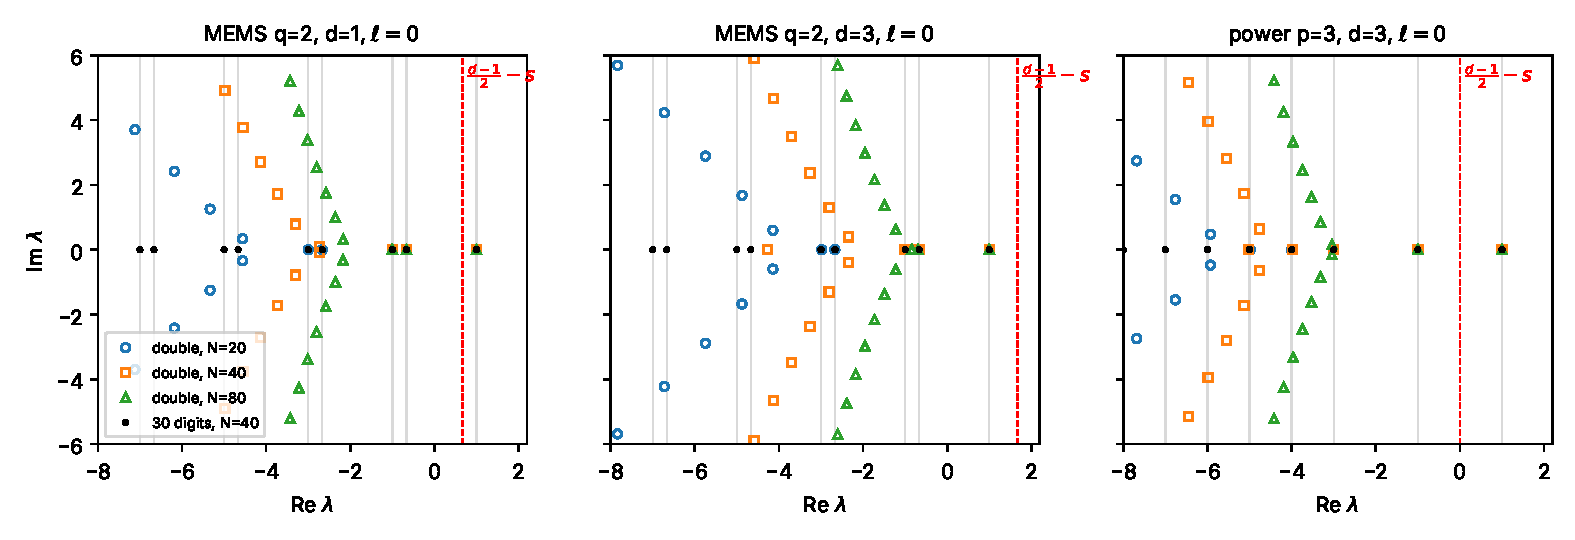
\includegraphics[width=\textwidth]{figures/num_spectra.pdf}
\caption{Eigenvalues of the collocation matrix of \eqref{num:eig}, $\ell=0$.
Coloured: double precision, $N=20,40,80$. Black dots: $30$-digit arithmetic,
$N=32$, which reproduce the closed form (grey vertical lines) exactly. The
red dashed line is $\operatorname{Re}\lambda=\frac{d-1}2-s$; the spurious
curve approaches it as $N$ grows.}
\label{num:fig-spec}
\end{figure}

%-----------------------------------------------------------------------------
\subsection{Touchdown dynamics of the hyperbolic MEMS equation}
\label{num:subsec-mems}

\paragraph{Problem and parameters.} We solve
\begin{equation}\label{num:mems}
  w_{tt}+\gamma w_t-\Delta w=-\lambda w^{-2}\ \text{ in }\Omega,\qquad
  w=1\text{ on }\partial\Omega,\qquad w(0)=1,\ w_t(0)=0,
\end{equation}
for $\Omega=(-1,1)$ and for radial solutions on the unit disk, with
$\gamma\in\{0,1\}$. The static pull-in value (fold of $\Delta w=\lambda w^{-2}$,
$w|_{\partial\Omega}=1$, by shooting) is $\lambda^*=0.35000$ ($d=1$) and $0.78923$
($d=2$); the dynamic threshold, defined as the smallest $\lambda$ with
$\min w<0.05$ before $t=30$, lies in $[0.2895,0.2961]$ ($d=1$, $\gamma=0$),
$[0.3426,0.3492]$ ($d=1$, $\gamma=1$), $[0.6406,0.6492]$ ($d=2$, $\gamma=0$) and
$[0.7438,0.7523]$ ($d=2$, $\gamma=1$) (\texttt{num\_mems\_threshold.py}; for $\gamma=0$
the finite-horizon value is an upper bound for the true threshold). We take
$\lambda=0.5$ ($d=1$) and $\lambda=0.8$ ($d=2$), above the dynamic threshold in all
four cases and small enough that the touchdown time exceeds $1$: for $T\le1$
the solution in $|x|<1-t$ is the ODE solution, and the gap closes
simultaneously on a whole interval (disk), a degenerate situation. With
$T>1$ the boundary has influenced the whole backward light cone of the
touchdown point.

\paragraph{A weak singularity.} The data are incompatible with the boundary
condition at second order ($w_{tt}(0)=-\lambda\ne0=\partial_t^2 1$), so a jump
of $w_{tt}$ travels inwards from $\partial\Omega$ along characteristics. In $d=2$
it focuses at $(t,r)=(1,0)$, i.e.\ \emph{inside} the backward light cone of
the touchdown point. This is physical (a voltage switched on instantaneously),
but it destroys the spectral accuracy of global methods: in a preliminary
test, a Chebyshev method in physical space changed $T$ by $\approx10^{-7}$
between $N=128$ and $N=256$. We
therefore use the following three-stage method.

\paragraph{Method.}
\emph{Stage 1 (physical space, $0\le t\le t_1$).} In $d=1$: leapfrog with
$\Delta t=\Delta x$ (exact for the free wave equation; the singular
characteristics are grid diagonals), on $M=4000,8000,16000$ cells, combined by
Richardson extrapolation; in $d=2$: the conservative second-order leapfrog for
$r^{-1}\partial_r(r\partial_r)$ with $\Delta t=\Delta r/2$, $M=4000,8000$, followed
by a least-squares fit of $w(t_1,\cdot)$, $w_t(t_1,\cdot)$ by even Chebyshev
polynomials of degree $40$ on $[0,R_0]$, which removes grid-scale noise
($\approx10^{-4}$ in $w_t$) left by the focusing; $R_0$ is kept below the
position of the singular front. The switching time $t_1$ is the multiple of
$0.01$ just before $\min w=0.3$.

\emph{Stage 2 (light cone of $(T,0)$, $t\ge t_1$).} With
$\tau=-\log\frac{T-t}{T-t_1}$, $\xi=\frac{x}{T-t}$, $\psi_1=(T-t)^{-2/3}w$,
$\psi_2=(T-t)^{1/3}w_t$,
\begin{equation}\label{num:simmems}
  \partial_\tau\psi_1=-\Lambda\psi_1+\tfrac23\psi_1+\psi_2,\qquad
  \partial_\tau\psi_2=\Delta\psi_1-\Lambda\psi_2-\tfrac13\psi_2-\lambda\psi_1^{-2}
  -\gamma(T-t_1)e^{-\tau}\psi_2 ,
\end{equation}
discretised by Chebyshev collocation in $\xi\in[-1,1]$ ($21$ nodes, $d=1$) or
in $z=|\xi|^2\in[0,1]$ ($17$ nodes, radial), without boundary conditions, and
integrated with an adaptive 8th-order Runge--Kutta method (DOP853, relative
tolerance $10^{-12}$). Initial data are interpolated from stage 1 (local
10-point Lagrange interpolation in $d=1$, the even fit in $d=2$). The ODE
profile is $(\psi_1,\psi_2)=(c,-\frac23c)$, $c=(9\lambda/2)^{1/3}$.

\emph{Stage 3 ($T$ by bisection).} If $T$ is too large, the solution quenches
inside the cone at finite $\tau$ ($\min\psi_1\to0$); if $T$ is too small,
$\psi_1\sim e^{2\tau/3}w(T,0)\to\infty$. Bisection is run to relative width
$4\cdot10^{-16}$. Because of the time-translation mode $e^{\tau}$, the two
trajectories belonging to the ends of the final bracket separate eventually;
all rates are measured only on the $\tau$-window where their values of
$W(\tau,0)-c$ agree to $0.1\%$.

\emph{Independent check.} Stage 1 alone, continued in physical space
($M=16000$, resp.\ $8000$) down to $\min w=0.02$ (resp.\ $0.03$), and fitted
with $T$ as a free parameter.

\paragraph{Results.} In all four cases the minimum of $w$ is attained at the
centre; the same holds for all values tested in \texttt{num\_mems\_threshold.py}
($\lambda=0.35,0.5,1$ for $d=1$, $\lambda=0.7,\dots,1.2$ for $d=2$, $\gamma=0,1$): no
off-centre or ring quenching occurred. The
main numbers are collected in \cref{num:tab-mems}; \cref{num:fig-mems,num:fig-mems2}
show the evolution.

\begin{table}[ht]
\centering\small
\setlength{\tabcolsep}{4pt}
\begin{tabular}{@{}lccccccc@{}}
\toprule
case & $T$ & $\min(T-t)$ & $\omega_{\rm fit}$ & $\omega$, $c$ free & $C_\infty/c-1$ & $\frac{\psi_2+\frac23c}{\psi_1-c}$ & rate of $\operatorname{osc}W$\\
\midrule
$d=1$, $\gamma=0$ & $1.75194263316$ & $1.2\cdot10^{-7}$ & $0.66663$ & $0.6649$ & $2.1\cdot10^{-7}$ & $-1.3319$ & $0.995$\\
$d=1$, $\gamma=1$ & $2.40507517419$ & $4.0\cdot10^{-8}$ & $0.66662$ & $0.6642$ & $2.6\cdot10^{-7}$ & $-1.3318$ & $0.994$\\
$d=2$, $\gamma=0$ & $1.41984985$ & $1.8\cdot10^{-7}$ & $0.66666$ & $0.6627$ & $1.2\cdot10^{-6}$ & $-1.3312$ & $0.991$\\
$d=2$, $\gamma=1$ & $2.214154$ & $2.6\cdot10^{-7}$ & $0.66655$ & $0.6597$ & $3.8\cdot10^{-6}$ & $-1.3296$ & $0.985$\\
\midrule
prediction & & & $\frac23$ & $\frac23$ & $0$ & $-\frac43$ & $1$\\
\bottomrule
\end{tabular}
\caption{Hyperbolic MEMS touchdown, $q=2$, $\lambda=0.5$ ($d=1$), $\lambda=0.8$
($d=2$). $T$: bisection (digits shown are stable under changes of the
light-cone resolution; in $d=2$ the stage-1 resolution changes $T$ by
$8\cdot10^{-9}$ ($\gamma=0$) and $2\cdot10^{-7}$ ($\gamma=1$)). $\min(T-t)$: end of
the validity window. $\omega_{\rm fit}$: fit of $W(\tau,0)-c$ by
$Ae^{-\omega\tau}+Be^{-\tau}+Ce^{-4\tau/3}$ on $\tau\ge3$ ($e^{-4\tau/3}$ is the
square of the gap mode); without the $C$ term one gets $0.6656$, $0.6651$,
$0.6643$, $0.6625$. Next column: fit $W(\tau,0)=C_\infty+Ae^{-\omega\tau}+Be^{-\tau}$
with $c$ unknown. Ratio column: at the end of the window, $\xi=0$. Last
column: decay rate of $\max_\xi W-\min_\xi W$.}
\label{num:tab-mems}
\end{table}

\begin{enumerate}[label=(\roman*),leftmargin=2em,itemsep=2pt]
\item \emph{Exponent and constant.} With $T$ from the bisection, the local
  slope $d\log w_{\min}/d\log(T-t)$ for $T-t<10^{-6}$ is $0.666656$,
  $0.666655$, $0.666640$, $0.666627$, and $w_{\min}(T-t)^{-2/3}\to c$; leaving $c$
  free in the fit returns $c=(9\lambda/2)^{1/3}$ to $2\cdot10^{-7}$ ($d=1$) and
  $4\cdot10^{-6}$ ($d=2$). The approach is slow: the relative correction is
  $(A/c)(T-t)^{2/3}$ with $A/c=-1.44,-2.18,-2.82,-3.87$, so that $w_{\min}$ is
  within $1\%$ of $c(T-t)^{2/3}$ only for $T-t\lesssim10^{-4}$--$6\cdot10^{-4}$, i.e.\
  $w_{\min}\lesssim3\cdot10^{-3}$--$10^{-2}$ (\cref{num:fig-mems}, middle;
  \cref{num:fig-mems2}, right).
  Consequently, the independent physical-space fits over $w_{\min}\in[0.02,0.25]$
  with $T$ free give $\beta=0.596,0.559,0.545,0.500$ for $w=C(T-t)^\beta$, and
  still $\beta=0.644,0.627,0.614,0.589$ if the correction
  $(1+e(T-t)^{2/3})$ is included; their $T$ deviates from the bisection value
  by $8\cdot10^{-5}$--$1.4\cdot10^{-3}$. \emph{Exponents read off from moderate gaps are
  biased low}; this matters when comparing with experiments or with
  simulations that stop at $w_{\min}=O(10^{-2})$.
\item \emph{Light-cone profile.} $W(t,\xi)=(T-t)^{-2/3}w(t,(T-t)\xi)$ converges
  uniformly on $|\xi|\le1$ to the constant $c$ (\cref{num:fig-mems2}, left), with
  $\|W-c\|_\infty\sim(T-t)^{\omega}$, $\omega=0.6666\pm0.0001$ when the
  quadratic term of the gap mode is included, in agreement with
  $\omega_0=\frac23$. The deviation is, to leading order, the spatially
  \emph{constant} eigenfunction $(1,-\frac43)$ of $\lambda=-\frac23$ (ratio column),
  i.e.\ the ODE-energy mode: $W(t,0)-c\approx A(T-t)^{2/3}$ with $A<0$, as for an
  ODE solution of negative energy. The spatial oscillation $\operatorname{osc}_\xi W$
  decays faster, like $(T-t)^{1}$, which is the next even eigenvalue
  $\lambda=-1$ (eigenfunction $1+\frac{|\xi|^2}{3d}$ in the first component). Damping does not change
  the rate (it enters at order $e^{-\tau}$), only the coefficients.
\end{enumerate}

\begin{figure}[ht]
\centering
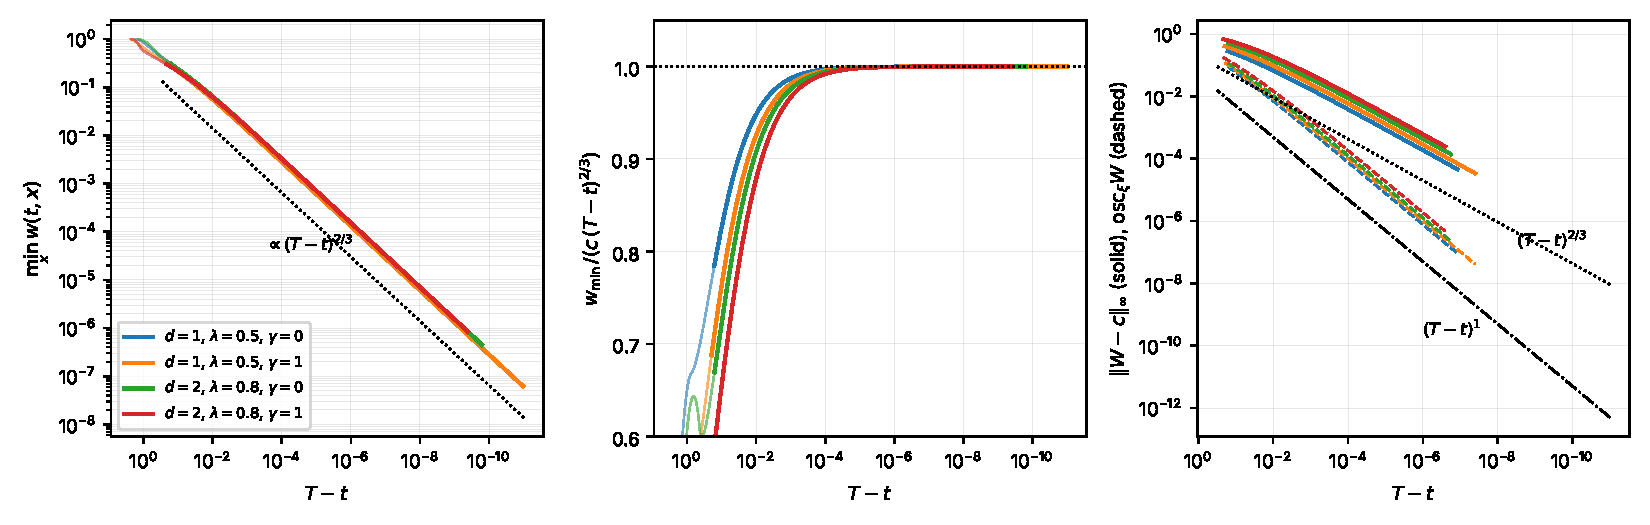
\includegraphics[width=\textwidth]{figures/num_mems_touchdown.pdf}
\caption{Hyperbolic MEMS touchdown. Left: $\min_xw$ versus $T-t$ (thin:
physical-space leapfrog alone; thick: light-cone evolution). Middle:
$w_{\min}/(c(T-t)^{2/3})$. Right: $\|W-c\|_{L^\infty(|\xi|\le1)}$ (solid) and
$\max_\xi W-\min_\xi W$ (dashed) with the slopes $\frac23$ and $1$.}
\label{num:fig-mems}
\end{figure}

\begin{figure}[ht]
\centering
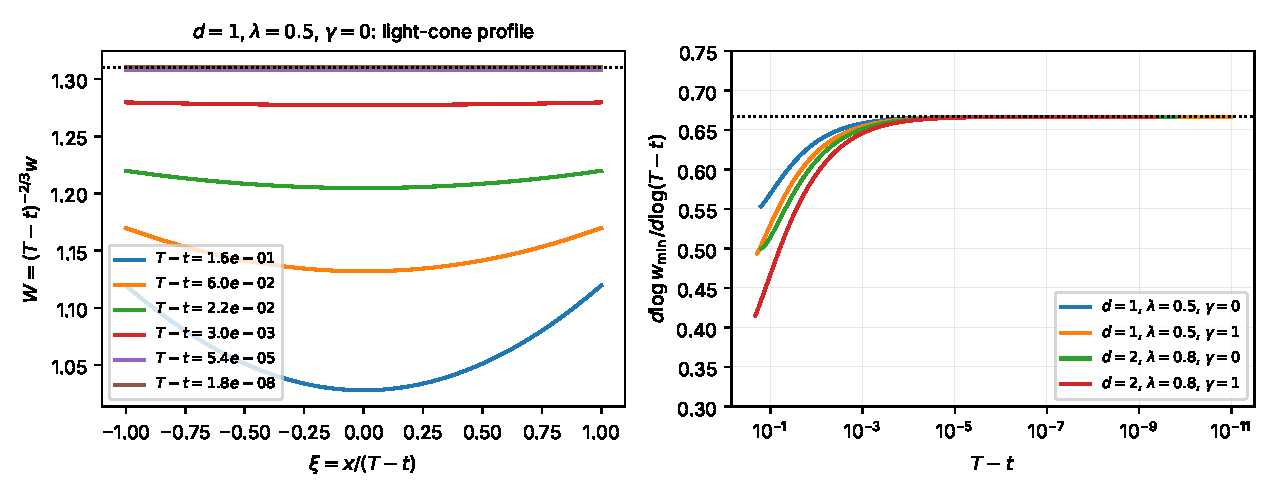
\includegraphics[width=0.85\textwidth]{figures/num_mems_profiles.pdf}
\caption{Left: light-cone profiles $W(t,\cdot)$, $d=1$, $\lambda=0.5$, $\gamma=0$,
flattening to $c$ (dotted). Right: local exponent $d\log w_{\min}/d\log(T-t)$.}
\label{num:fig-mems2}
\end{figure}

\paragraph{Comparison with \cite{GimperleinHeLacey2022}.} That work studies
the same equation formally and numerically for radial data and predicts
quenching at the origin with the ODE law $\kappa(T-t)^{2/(q+1)}$, stability of
this profile up to time translation, and instability of the non-trivial
self-similar profiles (as summarised in \cref{lit:sec}; we could not access
the full text, so we do not compare individual numbers). Our computations
agree on all three qualitative points: quenching at the centre, exponent
$\frac23$ and constant $(9\lambda/2)^{1/3}$, and convergence to the ODE profile
at the spectral-gap rate; starting from physical data we never observed an
approach to a non-trivial profile. Our computations add two quantitative points: the
identification of the slowest correction as the ODE-energy mode, and the
warning in (i) about pre-asymptotic exponents.

%-----------------------------------------------------------------------------
\subsection{Asymmetric data: flat or boosted profile?}
\label{num:subsec-boost}

The boosted family \eqref{fw:boost} reads, for MEMS,
$w=c(1-a^2)^{-\sigma/2}(T-t+a\cdot x)^{\sigma}$, i.e.\
$W_a(\xi)=c(1-a^2)^{-\sigma/2}(1+a\cdot\xi)^{\sigma}$ in the light cone. We
verified by substitution (\texttt{sympy}, $q=2,3,4$) that it is an exact
solution: with $Z=T-t+a\cdot x$, $w_{tt}-\Delta w=(1-|a|^2)W''(Z)$ and
$(1-|a|^2)W''+\lambda W^{-q}\equiv0$ for $W=c(1-|a|^2)^{-\sigma/2}Z^\sigma$.
As a test of the solver, $W_{0.4}$ stays stationary under \eqref{num:simmems}
to $4\cdot10^{-10}$ over $\tau\in[0,12]$ (the residual growth is the
time-translation instability seeded by round-off).

Since $W_a$ vanishes on the line $t=T+a(x-x_0)$, a boosted limit at a point
$x_0$ of the blowup curve $x\mapsto T(x)$ should have $a=T'(x_0)$ (in one
dimension and for power nonlinearities this is the Merle--Zaag picture of
non-characteristic points \cite{MerleZaag2007}); at the \emph{first}
touchdown point, $T'(x^*)=0$, and the profile should be flat. To test this we
took the asymmetric data $w(0,x)=1+0.25\,x(1-x^2)$, $w_t(0)=0$, $\lambda=0.5$,
$\gamma=0$, $d=1$, and computed by bisection, for twelve base points $x_0$, the
blowup time $T(x_0)$ of the backward light cone of $(T,x_0)$; this is the
blowup curve, which exists (and is $1$-Lipschitz) also beyond the first
touchdown, although the physical problem ends there.

\paragraph{Results.} The blowup curve (\cref{num:fig-boost}, left) is smooth
with a non-degenerate minimum at $x^*=0.00860$, $T(x^*)=1.7356545138$,
$T''(x^*)\approx1.76$: the asymmetric data shift the touchdown point (slightly
to the right, although the initial gap is smaller on the left), and
$|T'|\le0.23<1$ on the computed range, i.e.\ these points are non-characteristic. A degree-6 fit
through the twelve values of $T(x_0)$ (residual $7\cdot10^{-9}$; changing the
degree alters $T'$ by $<5\cdot10^{-5}$) gives $T'(x_0)$. At five base points the
boost parameter $a(t)$ of the light-cone profile, defined by
$W(t,1)/W(t,-1)=\big(\frac{1+a}{1-a}\big)^{2/3}$, converges, and at
$T(x_0)-t\approx6\cdot10^{-9}$:
\begin{center}\small
\begin{tabular}{@{}rrrrr@{}}
\toprule
$x_0-x^*$ & $a$ (light cone) & $T'(x_0)$ & $\|W-W_a\|_\infty$ & rate of $\|W-W_a\|_\infty$\\
\midrule
$0$ & $-0.0000112$ & $-0.0000116$ & $7.3\cdot10^{-6}$ & $0.654$\\
$-0.12$ & $-0.1981299$ & $-0.1981283$ & $6.2\cdot10^{-6}$ & $0.649$\\
$-0.06$ & $-0.1021323$ & $-0.1021325$ & $6.2\cdot10^{-6}$ & $0.650$\\
$+0.06$ & $+0.1096470$ & $+0.1096483$ & $8.1\cdot10^{-6}$ & $0.649$\\
$+0.12$ & $+0.2274879$ & $+0.2274882$ & $8.7\cdot10^{-6}$ & $0.647$\\
\bottomrule
\end{tabular}
\end{center}
(the rate is a straight-line fit of $\log\|W-W_{a(t)}\|_\infty$ against $\tau$ for $\tau>3$, which
is biased low by the same pre-asymptotic corrections as the two-term fits
quoted in the caption of \cref{num:tab-mems}; the window ends where the
trajectories for the two ends of the $T$-bracket differ by $10\%$ of
$\|W-W_a\|_\infty$). Thus $a_\infty=T'(x_0)$ to within $2\cdot10^{-6}$ at every
base point, and \emph{at the touchdown point the limit profile is the flat ODE
profile}: the residual $a\approx-1.1\cdot10^{-5}$ there is exactly $T'$ at
our numerical $x^*$, which is off by $\approx7\cdot10^{-6}$. Boosted
profiles appear only at points $x_0\neq x^*$ of the blowup curve, which the
physical (quenched) solution never reaches. For the stability theory this
means: the boost parameters must be modulated (the limit $a_\infty$ is not
determined by the symmetry of the data), but at the first touchdown point the
modulated parameter converges to $0$.

\begin{figure}[ht]
\centering
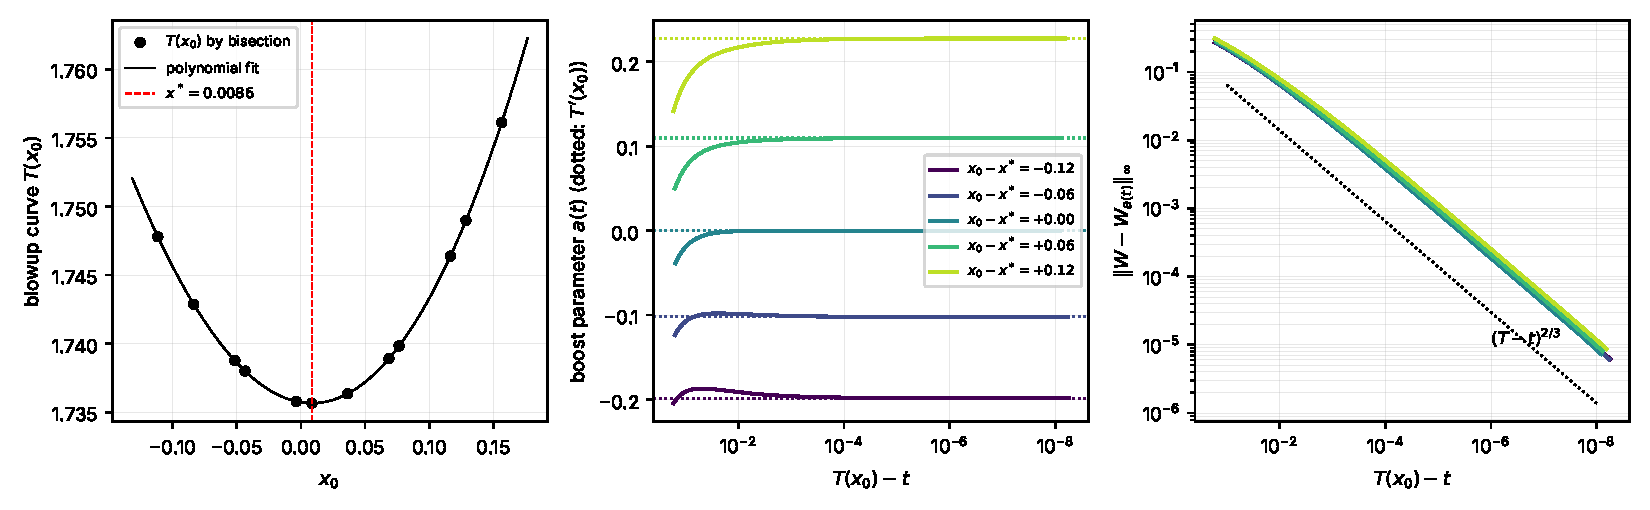
\includegraphics[width=\textwidth]{figures/num_mems_boost.pdf}
\caption{Asymmetric data $w(0,x)=1+0.25\,x(1-x^2)$, $\lambda=0.5$, $d=1$. Left:
blowup curve $T(x_0)$ (bisection) and the touchdown point $x^*$. Middle:
boost parameter of the light-cone profile at five base points versus
$T(x_0)-t$; dotted: $T'(x_0)$. Right: distance to the boosted family.}
\label{num:fig-boost}
\end{figure}

%-----------------------------------------------------------------------------
\subsection{Exponential nonlinearity in one dimension}
\label{num:subsec-exp}

The same three-stage method was applied to $u_{tt}-u_{xx}=e^u$ on $(-1,1)$,
$u=0$ at $x=\pm1$, $u(0)=u_t(0)=0$ (\texttt{num\_exp\_touchdown.py}; here
$\psi_1=u+2\log(T-t)$, $\psi_2=(T-t)u_t$, fixed point $(\log2,2)$; bisection
flags: $\max\psi_1\to\infty$ if $T$ is too large, $\psi_1\to-\infty$ if too small).
Blowup occurs at $x=0$ at $T=2.91356673558862$ (switching time $t_1=2.68$; the
value changes by $1.7\cdot10^{-13}$ if the light-cone resolution is increased).
Here \cref{num:tab-spec} predicts, in the even sector, the eigenvalues $1$
(time translation), $-1$ with eigenfunction $(1-\xi^2,\,-(1+\xi^2))$ and $-2$
(constant, the ODE energy mode), so the deviation should decay like
$(T-t)^1$ with the shape $1-\xi^2$. Measured: $\omega=1.00000$ (fit
$Ae^{-\omega\tau}+Be^{-2\tau}$ on $\tau\in[3,12.1]$; late-window slope
$0.99996$); at $T-t=1.3\cdot10^{-6}$ the deviation is
$\psi_1-\log2\propto 1-1.0004\,\xi^2+5\cdot10^{-7}\xi^4$, and
$(\psi_2-2)/(\psi_1(\cdot,0)-\log2)=-1.0008$ at $\xi=0$ and $-2.0012$ at $\xi=\pm1$
(predicted $-1$, $-2$; the small offsets are the time-translation mode
$(1,1)$ seeded by round-off); see \cref{num:fig-exp}. Note that, unlike MEMS with
$q=2$, the slowest mode is \emph{not} spatially constant: the ODE energy mode
($-2$) is faster than the first spatial mode ($-1$).

\begin{figure}[ht]
\centering
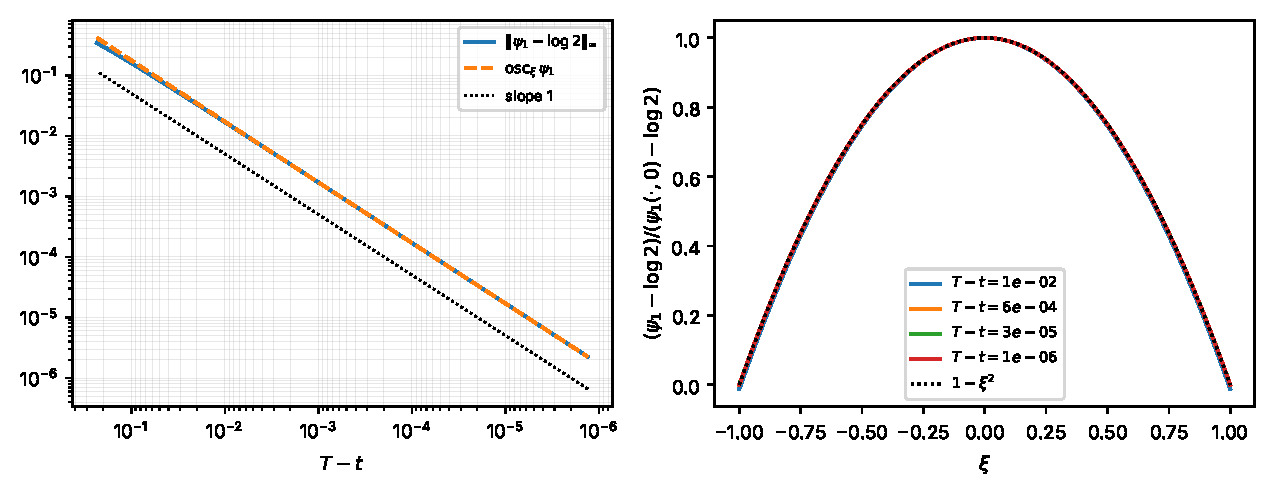
\includegraphics[width=0.8\textwidth]{figures/num_exp_touchdown.pdf}
\caption{$u_{tt}-u_{xx}=e^u$: deviation from the ODE profile in the light cone
(left) and its shape (right), normalised at $\xi=0$, versus $1-\xi^2$.}
\label{num:fig-exp}
\end{figure}

%-----------------------------------------------------------------------------
\subsection{Discrepancies, caveats and reproducibility}
\label{num:subsec-repro}

\paragraph{Discrepancies with the analytic hints.}
\begin{enumerate}[leftmargin=1.6em,itemsep=1pt]
\item MEMS $q=3$ (and $p=5$): Jordan blocks at the collisions of the two
  eigenvalue families, including the gap eigenvalue $\lambda=-1$ for $q=3$
  (\ref{num:D-jordan}). Semisimplicity, which the hint asks to check, holds for
  $\lambda=1$ and $\lambda=0$ in all cases, but fails there.
\item The derivative model is outside the scope of \eqref{fw:eig}
  (\ref{num:D-deriv}); its spectrum is the free one with $s=-1$.
\item The closed-form lists are exact for polynomial eigenfunctions, but their
  meaning as $\mathcal H^k$-spectra requires $k\ge\frac d2-s+\omega_0$
  (\ref{num:D-buried}); the energy space is too small for MEMS in every
  dimension.
\item No discrepancy in the nonlinear tests: exponent $\frac23$, constant
  $(9\lambda/2)^{1/3}$, rate $\omega_0=\frac23$ (MEMS), $\omega_0=1$ ($e^u$) and flat
  limit at the touchdown point are all confirmed. The hint that the profile
  ``can also converge to a boosted profile'' is correct only at points $x_0\neq x^*$
  of the blowup curve, with $a=T'(x_0)$.
\end{enumerate}

\paragraph{Caveats.}
\begin{itemize}[leftmargin=1.4em,itemsep=1pt]
\item The eigenvalue computations only probe polynomial eigenfunctions
  (\cref{num:prop-tri}); absence of non-polynomial eigenfunctions in
  $\operatorname{Re}\lambda>-\omega_k$ rests on the connection-formula
  argument of \cref{fw:thm-spec}, not on numerics.
\item The nonlinear simulations cover one $\lambda$ per geometry, $q=2$, and
  data at rest; the light-cone stage is spectrally accurate, but the data at
  $t_1$ carry errors of $10^{-10}$--$3\cdot10^{-8}$ ($d=1$) and up to $10^{-7}$
  ($w$) and $2\cdot10^{-5}$ ($w_t$) in $d=2$ because of the corner singularity;
  these shift $T$ (by up to $2\cdot10^{-7}$ in $d=2$) but not the measured rates.
\item Rates are measured on windows of $12$--$17$ units of $\tau$ (5--7 decades
  of $T-t$), limited by the time-translation instability amplifying
  integration errors of size $\approx10^{-14}$.
\item The dynamic pull-in values for $\gamma=0$ are finite-horizon ($t\le30$) values.
\item We could not access the full text of \cite{GimperleinHeLacey2022}
  (network restrictions); the comparison above is with the summary of that
  work in \cref{lit:sec}.
\end{itemize}

\paragraph{Reproducibility.} All scripts run from the project root with
\texttt{python3 code/<name>.py} (numpy, scipy, sympy, mpmath, matplotlib);
times are wall-clock times on a shared 4-core machine.
\begin{center}\small
\begin{tabular}{@{}lll@{}}
\toprule
script & output & time\\
\midrule
\texttt{num\_spectra.py} & \cref{num:tab-spec}, \cref{num:fig-spec}, eigenvector checks & $\approx4$ min\\
\texttt{num\_spurious.py} & spurious-branch edges $K_N$ (\cref{num:subsec-spec}) & $<1$ min\\
\texttt{num\_mems\_threshold.py} & pull-in values, location of the minimum & $<1$ min\\
\texttt{num\_mems\_touchdown.py} & \cref{num:tab-mems}, \cref{num:fig-mems,num:fig-mems2} & $\approx4$--$5$ min\\
\texttt{num\_mems\_boost.py} & \cref{num:fig-boost} and the boost table & $\approx4$ min\\
\texttt{num\_exp\_touchdown.py} & \cref{num:fig-exp} & $<1$ min\\
\texttt{num\_common.py} & shared solvers (not run directly) & ---\\
\bottomrule
\end{tabular}
\end{center}

